\documentclass{article}
\usepackage{graphicx} % Required for inserting images

\title{Homework 3}
\author{Ayman Tawaalai }
\date{January 2024}

\begin{document}

\maketitle

\section{Introduction}
The purpose of the given assignment is to study and implement logistic regression through practical means. The assignment states that the student must one hot encode and ngram the patient sequence data from homework 1. Once that is completed, it will serve as the vectors for logistic regression. Logistic regression must be implemented manually without the use of external libraries.

\section{Logistic Regression}
Logistic regression is a supervised learning model that determines whether something is true or false based on a logistic function. The function creates an S curve where the center is 50\% and items above go from 51 to 100 while below go from 1 to 49. Based on where the x value is based will determine the probability of a categorical outcome. This is done through the use of the sigmoid function which will be implemented in the python implementation.

\section{Implementation}
To implement logistic regression the first step would be to take in the data set. Since all the patient data files are in the ".file" extension, pandas is used to read them as csv's and then place them in a data frame. Since the categorical data being measured is in the third column, one hot encoding is done on the third column. 
\begin{figure}
    \centering
    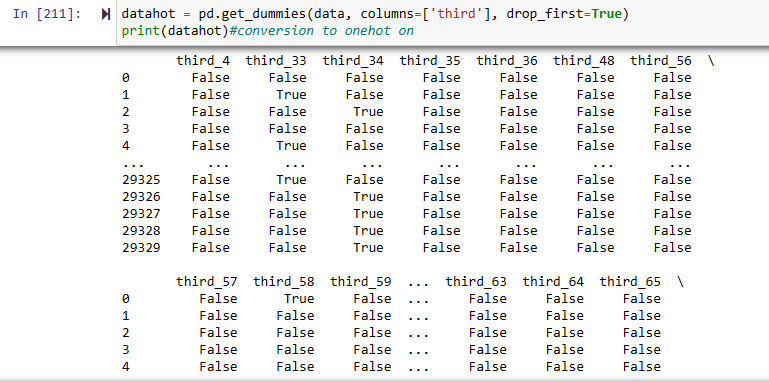
\includegraphics[width=0.5\linewidth]{a.png}
    \caption{One Hot Encoding}
    \label{fig:enter-label}
\end{figure}
After on hot encoding is complete, the next step would be to conduct ngram. Ngram would by recieving the total amount of "grams", essentially the break up, and goes through each set of given data using the gram. To implement it in python, the method getngrams will be used. It will take in the dataset of a one hot and then attain the starting point to n and will continue this process until the dataset is completed.
\begin{figure}
    \centering
    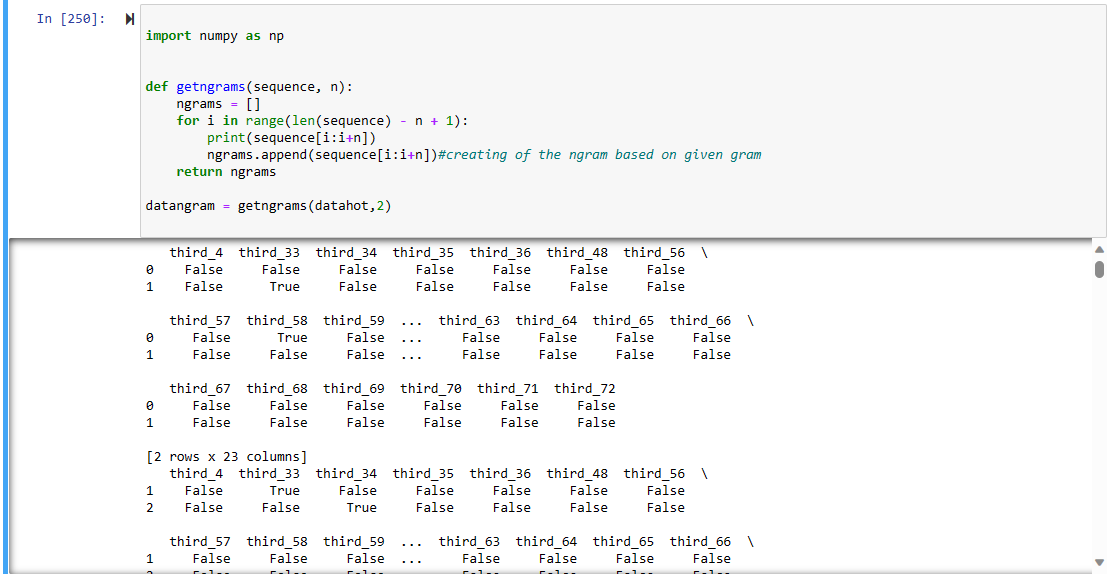
\includegraphics[width=0.5\linewidth]{b.png}
    \caption{NGram}
    \label{fig:enter-label}
\end{figure}


The next step would be to create labels for learning, x, and y arrays that will be fed into the model. Within the yarr a label must be selected. These labels are from the column names in one hot. Within the logisticreg function houses the model itself. Initialization is done to set biases and set the field for the model to replace items within. The while loop will call on the sigmoid function to conduct this regression. It will send the current array of x datahot values along with theta to plug into the equation. It will send back an array where gradient descent will be calculated. The product of the gradient descent and the user entered learning rate will become the new theta. The loss will also be calculated and compared to the user entered threshold to know when the loop can stop.
\begin{figure}
    \centering
    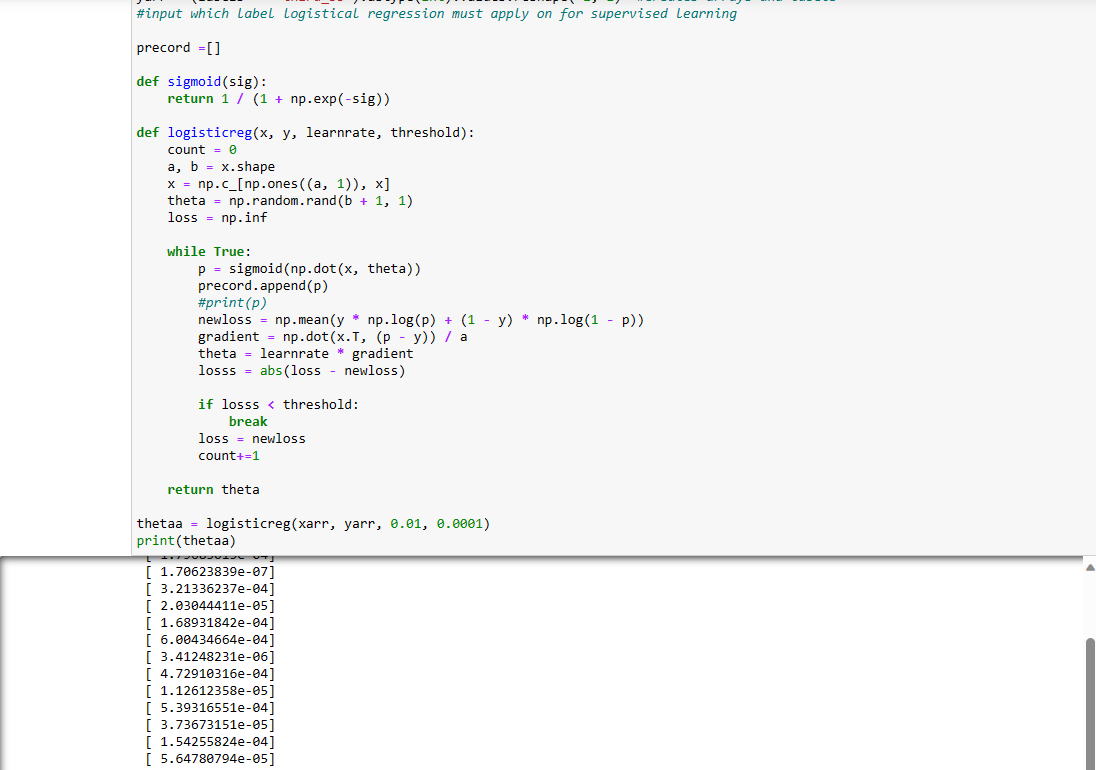
\includegraphics[width=0.5\linewidth]{c.png}
    \caption{Logistic Regression Model}
    \label{fig:enter-label}
\end{figure}

\section{Weka}
Modification to the datafram were needed to place it in weka. Once loaded in Weka the summary gave unsavory results. The high mean squared error and relative absolute error would, at first glance, show that this model does not fit well with the dataset. This is because the loaded dataset was the one hot encoding and this could result in the errors below. Furthermore it will also depend on what label is used in the model. 
=== Summary ===

Correlation coefficient                  0.0806
Mean absolute error                      0.007 
Root mean squared error                  0.0563
Relative absolute error                108.9886 %
Root relative squared error             99.6719 %
Total Number of Instances            29330    
\section{Conclusion}
The purpose of the assignment was to implement logistic regression from scratch to better understand how the model works. While the python implementation provided what was asked for, weka's provided information shows that this model is may have issues based on the one hot that was passed into it. However, this can be variable based on the selected label.
\end{document}
